% Created by tikzDevice version 0.9 on 2016-02-03 14:00:39
% !TEX encoding = UTF-8 Unicode
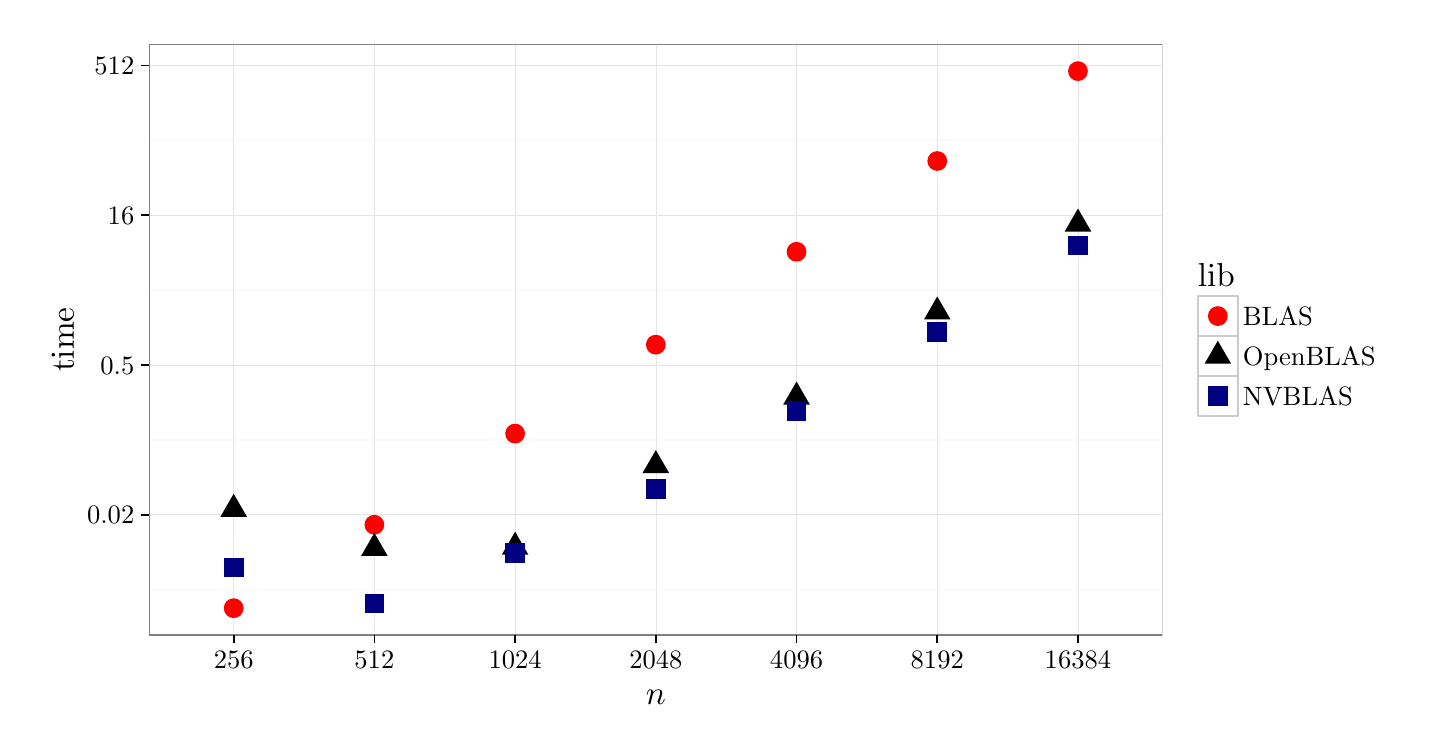
\begin{tikzpicture}[x=1pt,y=1pt]
\definecolor{fillColor}{RGB}{255,255,255}
\path[use as bounding box,fill=fillColor,fill opacity=0.00] (0,0) rectangle (505.89,252.94);
\begin{scope}
\path[clip] (  0.00,  0.00) rectangle (505.89,252.94);
\definecolor{drawColor}{RGB}{255,255,255}
\definecolor{fillColor}{RGB}{255,255,255}

\path[draw=drawColor,line width= 0.6pt,line join=round,line cap=round,fill=fillColor] (  0.00,  0.00) rectangle (505.89,252.95);
\end{scope}
\begin{scope}
\path[clip] ( 43.93, 33.48) rectangle (410.03,246.94);
\definecolor{fillColor}{RGB}{255,255,255}

\path[fill=fillColor] ( 43.93, 33.48) rectangle (410.03,246.94);
\definecolor{drawColor}{gray}{0.98}

\path[draw=drawColor,line width= 0.6pt,line join=round] ( 43.93, 49.87) --
	(410.03, 49.87);

\path[draw=drawColor,line width= 0.6pt,line join=round] ( 43.93,103.99) --
	(410.03,103.99);

\path[draw=drawColor,line width= 0.6pt,line join=round] ( 43.93,158.11) --
	(410.03,158.11);

\path[draw=drawColor,line width= 0.6pt,line join=round] ( 43.93,212.24) --
	(410.03,212.24);
\definecolor{drawColor}{gray}{0.90}

\path[draw=drawColor,line width= 0.2pt,line join=round] ( 43.93, 76.93) --
	(410.03, 76.93);

\path[draw=drawColor,line width= 0.2pt,line join=round] ( 43.93,131.05) --
	(410.03,131.05);

\path[draw=drawColor,line width= 0.2pt,line join=round] ( 43.93,185.17) --
	(410.03,185.17);

\path[draw=drawColor,line width= 0.2pt,line join=round] ( 43.93,239.30) --
	(410.03,239.30);

\path[draw=drawColor,line width= 0.2pt,line join=round] ( 74.44, 33.48) --
	( 74.44,246.94);

\path[draw=drawColor,line width= 0.2pt,line join=round] (125.28, 33.48) --
	(125.28,246.94);

\path[draw=drawColor,line width= 0.2pt,line join=round] (176.13, 33.48) --
	(176.13,246.94);

\path[draw=drawColor,line width= 0.2pt,line join=round] (226.98, 33.48) --
	(226.98,246.94);

\path[draw=drawColor,line width= 0.2pt,line join=round] (277.83, 33.48) --
	(277.83,246.94);

\path[draw=drawColor,line width= 0.2pt,line join=round] (328.68, 33.48) --
	(328.68,246.94);

\path[draw=drawColor,line width= 0.2pt,line join=round] (379.52, 33.48) --
	(379.52,246.94);
\definecolor{fillColor}{RGB}{255,0,0}

\path[fill=fillColor] ( 74.44, 43.18) circle (  3.57);

\path[fill=fillColor] (125.28, 73.32) circle (  3.57);

\path[fill=fillColor] (176.13,106.26) circle (  3.57);

\path[fill=fillColor] (226.98,138.39) circle (  3.57);

\path[fill=fillColor] (277.83,171.97) circle (  3.57);

\path[fill=fillColor] (328.68,204.76) circle (  3.57);

\path[fill=fillColor] (379.52,237.24) circle (  3.57);
\definecolor{fillColor}{RGB}{0,0,0}

\path[fill=fillColor] ( 74.44, 84.51) --
	( 79.24, 76.19) --
	( 69.63, 76.19) --
	cycle;

\path[fill=fillColor] (125.28, 70.38) --
	(130.09, 62.05) --
	(120.48, 62.05) --
	cycle;

\path[fill=fillColor] (176.13, 70.81) --
	(180.94, 62.48) --
	(171.33, 62.48) --
	cycle;

\path[fill=fillColor] (226.98,100.33) --
	(231.79, 92.00) --
	(222.17, 92.00) --
	cycle;

\path[fill=fillColor] (277.83,125.07) --
	(282.63,116.75) --
	(273.02,116.75) --
	cycle;

\path[fill=fillColor] (328.68,155.81) --
	(333.48,147.49) --
	(323.87,147.49) --
	cycle;

\path[fill=fillColor] (379.52,187.59) --
	(384.33,179.26) --
	(374.72,179.26) --
	cycle;
\definecolor{fillColor}{RGB}{0,0,128}

\path[fill=fillColor] ( 70.87, 54.26) --
	( 78.00, 54.26) --
	( 78.00, 61.40) --
	( 70.87, 61.40) --
	cycle;

\path[fill=fillColor] (121.72, 41.26) --
	(128.85, 41.26) --
	(128.85, 48.39) --
	(121.72, 48.39) --
	cycle;

\path[fill=fillColor] (172.56, 59.42) --
	(179.70, 59.42) --
	(179.70, 66.56) --
	(172.56, 66.56) --
	cycle;

\path[fill=fillColor] (223.41, 82.80) --
	(230.55, 82.80) --
	(230.55, 89.94) --
	(223.41, 89.94) --
	cycle;

\path[fill=fillColor] (274.26,110.85) --
	(281.40,110.85) --
	(281.40,117.99) --
	(274.26,117.99) --
	cycle;

\path[fill=fillColor] (325.11,139.48) --
	(332.24,139.48) --
	(332.24,146.61) --
	(325.11,146.61) --
	cycle;

\path[fill=fillColor] (375.96,170.68) --
	(383.09,170.68) --
	(383.09,177.81) --
	(375.96,177.81) --
	cycle;
\definecolor{drawColor}{gray}{0.50}

\path[draw=drawColor,line width= 0.6pt,line join=round,line cap=round] ( 43.93, 33.48) rectangle (410.03,246.94);
\end{scope}
\begin{scope}
\path[clip] (  0.00,  0.00) rectangle (505.89,252.94);
\definecolor{drawColor}{RGB}{0,0,0}

\node[text=drawColor,anchor=base east,inner sep=0pt, outer sep=0pt, scale=  0.96] at ( 38.53, 73.62) {0.02};

\node[text=drawColor,anchor=base east,inner sep=0pt, outer sep=0pt, scale=  0.96] at ( 38.53,127.75) {0.5};

\node[text=drawColor,anchor=base east,inner sep=0pt, outer sep=0pt, scale=  0.96] at ( 38.53,181.87) {16};

\node[text=drawColor,anchor=base east,inner sep=0pt, outer sep=0pt, scale=  0.96] at ( 38.53,235.99) {512};
\end{scope}
\begin{scope}
\path[clip] (  0.00,  0.00) rectangle (505.89,252.94);
\definecolor{drawColor}{RGB}{0,0,0}

\path[draw=drawColor,line width= 0.6pt,line join=round] ( 40.93, 76.93) --
	( 43.93, 76.93);

\path[draw=drawColor,line width= 0.6pt,line join=round] ( 40.93,131.05) --
	( 43.93,131.05);

\path[draw=drawColor,line width= 0.6pt,line join=round] ( 40.93,185.17) --
	( 43.93,185.17);

\path[draw=drawColor,line width= 0.6pt,line join=round] ( 40.93,239.30) --
	( 43.93,239.30);
\end{scope}
\begin{scope}
\path[clip] (  0.00,  0.00) rectangle (505.89,252.94);
\definecolor{drawColor}{RGB}{0,0,0}

\path[draw=drawColor,line width= 0.6pt,line join=round] ( 74.44, 30.48) --
	( 74.44, 33.48);

\path[draw=drawColor,line width= 0.6pt,line join=round] (125.28, 30.48) --
	(125.28, 33.48);

\path[draw=drawColor,line width= 0.6pt,line join=round] (176.13, 30.48) --
	(176.13, 33.48);

\path[draw=drawColor,line width= 0.6pt,line join=round] (226.98, 30.48) --
	(226.98, 33.48);

\path[draw=drawColor,line width= 0.6pt,line join=round] (277.83, 30.48) --
	(277.83, 33.48);

\path[draw=drawColor,line width= 0.6pt,line join=round] (328.68, 30.48) --
	(328.68, 33.48);

\path[draw=drawColor,line width= 0.6pt,line join=round] (379.52, 30.48) --
	(379.52, 33.48);
\end{scope}
\begin{scope}
\path[clip] (  0.00,  0.00) rectangle (505.89,252.94);
\definecolor{drawColor}{RGB}{0,0,0}

\node[text=drawColor,anchor=base,inner sep=0pt, outer sep=0pt, scale=  0.96] at ( 74.44, 21.46) {256};

\node[text=drawColor,anchor=base,inner sep=0pt, outer sep=0pt, scale=  0.96] at (125.28, 21.46) {512};

\node[text=drawColor,anchor=base,inner sep=0pt, outer sep=0pt, scale=  0.96] at (176.13, 21.46) {1024};

\node[text=drawColor,anchor=base,inner sep=0pt, outer sep=0pt, scale=  0.96] at (226.98, 21.46) {2048};

\node[text=drawColor,anchor=base,inner sep=0pt, outer sep=0pt, scale=  0.96] at (277.83, 21.46) {4096};

\node[text=drawColor,anchor=base,inner sep=0pt, outer sep=0pt, scale=  0.96] at (328.68, 21.46) {8192};

\node[text=drawColor,anchor=base,inner sep=0pt, outer sep=0pt, scale=  0.96] at (379.52, 21.46) {16384};
\end{scope}
\begin{scope}
\path[clip] (  0.00,  0.00) rectangle (505.89,252.94);
\definecolor{drawColor}{RGB}{0,0,0}

\node[text=drawColor,anchor=base,inner sep=0pt, outer sep=0pt, scale=  1.20] at (226.98,  8.40) {$n$};
\end{scope}
\begin{scope}
\path[clip] (  0.00,  0.00) rectangle (505.89,252.94);
\definecolor{drawColor}{RGB}{0,0,0}

\node[text=drawColor,rotate= 90.00,anchor=base,inner sep=0pt, outer sep=0pt, scale=  1.20] at ( 16.66,140.21) {time};
\end{scope}
\begin{scope}
\path[clip] (  0.00,  0.00) rectangle (505.89,252.94);
\definecolor{fillColor}{RGB}{255,255,255}

\path[fill=fillColor] (418.57,108.32) rectangle (491.35,172.10);
\end{scope}
\begin{scope}
\path[clip] (  0.00,  0.00) rectangle (505.89,252.94);
\definecolor{drawColor}{RGB}{0,0,0}

\node[text=drawColor,anchor=base west,inner sep=0pt, outer sep=0pt, scale=  1.20] at (422.84,159.57) {lib};
\end{scope}
\begin{scope}
\path[clip] (  0.00,  0.00) rectangle (505.89,252.94);
\definecolor{drawColor}{gray}{0.80}
\definecolor{fillColor}{RGB}{255,255,255}

\path[draw=drawColor,line width= 0.6pt,line join=round,line cap=round,fill=fillColor] (422.84,141.50) rectangle (437.29,155.95);
\end{scope}
\begin{scope}
\path[clip] (  0.00,  0.00) rectangle (505.89,252.94);
\definecolor{fillColor}{RGB}{255,0,0}

\path[fill=fillColor] (430.06,148.73) circle (  3.57);
\end{scope}
\begin{scope}
\path[clip] (  0.00,  0.00) rectangle (505.89,252.94);
\definecolor{drawColor}{gray}{0.80}
\definecolor{fillColor}{RGB}{255,255,255}

\path[draw=drawColor,line width= 0.6pt,line join=round,line cap=round,fill=fillColor] (422.84,127.04) rectangle (437.29,141.50);
\end{scope}
\begin{scope}
\path[clip] (  0.00,  0.00) rectangle (505.89,252.94);
\definecolor{fillColor}{RGB}{0,0,0}

\path[fill=fillColor] (430.06,139.82) --
	(434.87,131.50) --
	(425.26,131.50) --
	cycle;
\end{scope}
\begin{scope}
\path[clip] (  0.00,  0.00) rectangle (505.89,252.94);
\definecolor{drawColor}{gray}{0.80}
\definecolor{fillColor}{RGB}{255,255,255}

\path[draw=drawColor,line width= 0.6pt,line join=round,line cap=round,fill=fillColor] (422.84,112.59) rectangle (437.29,127.04);
\end{scope}
\begin{scope}
\path[clip] (  0.00,  0.00) rectangle (505.89,252.94);
\definecolor{fillColor}{RGB}{0,0,128}

\path[fill=fillColor] (426.50,116.25) --
	(433.63,116.25) --
	(433.63,123.39) --
	(426.50,123.39) --
	cycle;
\end{scope}
\begin{scope}
\path[clip] (  0.00,  0.00) rectangle (505.89,252.94);
\definecolor{drawColor}{RGB}{0,0,0}

\node[text=drawColor,anchor=base west,inner sep=0pt, outer sep=0pt, scale=  0.96] at (439.10,145.42) {BLAS};
\end{scope}
\begin{scope}
\path[clip] (  0.00,  0.00) rectangle (505.89,252.94);
\definecolor{drawColor}{RGB}{0,0,0}

\node[text=drawColor,anchor=base west,inner sep=0pt, outer sep=0pt, scale=  0.96] at (439.10,130.97) {OpenBLAS};
\end{scope}
\begin{scope}
\path[clip] (  0.00,  0.00) rectangle (505.89,252.94);
\definecolor{drawColor}{RGB}{0,0,0}

\node[text=drawColor,anchor=base west,inner sep=0pt, outer sep=0pt, scale=  0.96] at (439.10,116.51) {NVBLAS};
\end{scope}
\end{tikzpicture}
